
\chapter{Introduction}
\raggedbottom
\clearpage
\section{Background}
The upper, sunlight region of the pelagic ocean, or ``euphotic'' zone, is home to microscopic plants, phytoplankton, which in this well-lit environment thrive and photosynthesize. Though individually quite small, the combined net primary production (NPP) of this diverse consortium in the marine system is estimated to be 48.5 Pg of carbon (C) per year, nearly 50\% of global NPP \citep{Longhurst1995, Field1998}. Due to this significant role in the carbon cycle, the identification of the major factors controlling phytoplankton ecology, physiology, and, ultimately, bloom dynamics has been a central problem in the field of biological oceanography for the past century. From physical explanations (Sverdrup's critical depth hypothesis \citep{Sverdrup1953}), to chemical rationale (Redfield ratio \citep{Redfield1958}), to ecological theory (Margalef's mandala \citep{Margalef1978}), the field has been constantly reevaluating evidence to answer the question: What drives phytoplankton production?\par

Since these foundational hypotheses were put forth, significant advancements in the study of ocean primary production have been made both through the continued collection of traditional biological oceanographic datasets (e.g. chlorophyll, nutrients, taxonomic counts) particularly at long-term sampling sites \citep{Karl1996, Steinberg2001,Smith2003, Li1998}, and through technological advancements. Remote sensing from satellites, starting with radiometric with the Coastal Zone Color Scanner (CZCS) in 1978, enabled global-scale estimates of chlorophyll \textit{a} and spawned a new generation of missions to measure ocean color (e.g. SeaWiFs, MODIS Aqua) \citep{McClain2009}. High-throughput approaches such as flow cytometry, the early use of which led to the discovery of the most abundant photosynthetic organism on Earth \citep{Chisholm1988}, have now been expand to enable automated measurements along oceanic transects \citep{Swalwell2011, Ribalet2015} and over time series \citep{Olson2003}. The integration of molecular techniques into the study of marine microbes has provided a window into this previously muddled and complex world. With these tools we have discovered previously unknown diversity in the plankton \citep{Lopez-Garcia2001}, clarified the evolutionary histories of protists \citep{Keeling2005}, characterized previously invisible microbial communities \citep{Fuhrman1993}, and tracked the molecular metabolism underlying biogeochemical cycles \citep{Konneke2005}. Despite the impressive advances that have been made in assessing the diversity of marine microorganisms, the mechanisms that underlie the participation of microorganisms in marine food webs and biogeochemical cycles are poorly understood.

The macronutrients nitrogen (N) and phosphorus (P) are widely recognized to be major drivers of phytoplankton growth and activities in marine systems \citep{}. In many regards, however, we lack a fundamental understanding of how nutrients are metabolized by different phytoplankton species and functional groups: processes that may directly dictate their distributions and activities. Characterizing the interplay between individual phytoplankton taxa and their N and P environment in a natural setting remains a major on-going challenge, as many metrics such as elemental composition or enzymatic activity lack specificity and can largely only be assessed for the bulk community. These studies may be taken in to the lab, but doing so limits the ability to truly compare between species as you can in a natural setting where organisms all exist within the same complex environment. This thesis will focus on the following questions:


\begin{enumerate}
  \item How do phytoplankton respond to changing (light, nutrient, temperature) environments? Are these changes common across functional groups, genera, species, strains? 
  \item What enables the maintenance of diverse phytoplankton communities? 
  \item How does diversity (genetic, functional) influence ecosystem function and biogeochemical cycling? 
      
\end{enumerate}

Using a combination of field and experimental approaches, and harnessing new molecular tools, this thesis aims to address these questions at a detailed, molecular-level. 

\subsection{Eukaryotic phytoplankton are diverse}


Photosynthetic organisms at the broadest level can be broken into two distinct groups: prokaryotes (primarily bacteria\footnote{There are some organisms currently classified as archaea that are phototrophs (e.g. the haloarchaeon \textit{Haloarcula marismortui}). However, these organisms do not fix carbon and rely upon bacteriorhodopsin rather than chlorophyll. To date, chlorophyll biosynthesis has not been detected in archaea \citep{Bryant2006}.} and eukaryotes. While, cyanobacteria are numerically more abundant, this thesis will focus on the larger, eukaryotic fraction of photosynthetic plankton. All eukaryotic photosynthetic organisms (terrestrial and marine) are believed to have descended from one common ancestor and then diversified into three main lineages: green algae, glaucophytes, and red algae \citep{Falkowski2004}. Land plants are significantly more diverse at the species-level (\textasciitilde268,600 species)\citep{Chapman2009} than are phytoplankton (\textasciitilde25,000) \citep{Costello2013}. However, unlike land plants, which are a ``crown'' group, classified within a single clade --- Virdiplantae, algae span all three of the photosynthetic eukaryotic groupings and are far more genetically diverse as a whole, then are land plants \citep{Falkowski2004}.  
\par
Thus phytoplankton are integrally tied to the geochemistry of the world's oceans, just as the geochemistry of the ocean is tied to them. 


{How important is diversity?}

\subsection{Molecular tools to shed light on mixed communities}

As with the field of medicine, advances in sequencing and mass spectrometry technologies over the last decade have accelerated investigations of diversity and function the field of biological oceanography. The burgeoning technologies fueling the ``-omics''\footnote{``-omics'' is a catch-all suffix typically used to describe large, molecular datasets (e.g. genomics, the study of the genome, and transcriptomics, the study of the complete set of RNA transcripts produced under certain conditions). The use of this suffix, however, is expanding to other fields (see \href{https://twitter.com/search?q=\%23badomics&src=typd&lang=en}{\#badomics}). } revolution allow a unique glimpse at the previously hidden molecular world of the microbes, enabling the tracking of species-specific metabolism in the environment. \par

Molecular techniques are an effective means to identify differences in physiological ecology in marine microbes (Doney et al., 2004) through genomic (Gobler et al., 2011; Rocap et al., 2003), transcriptomic (Wurch et al., 2011;Dyhrman et al., 2012), metagenomic (Johnson et al., 2006; Coleman and Chisholm, 2010), and, more recently, metatranscriptomic approaches (Gifford et al., 2012). Translating molecular-level measures of physiological ecology into defined differences in niche space remains a challenge. Metatranscriptomic studies present the unique opportunity to distinguish the active partitioning of niches by organisms in the environment, as opposed to evolutionary markers of partitioned niches observed with metagenomic studies. As such, metatranscriptomics can be applied in a quantitative context to identify the realized niche of a species and illuminate the species-specific niche partitioning strategies operating in the environment.

Brynn's study of the interplay between marine microbes and diatom hosts: illuminating connections not before seen. 
Particle associated bacteria (stravinksi)
Ottensen diel cycling
Genomic diversity with single celled genomes
Mak saito paper on proteomics

\section{Objective and Outline}
The overarching goal of this thesis was to develop bioinformatic tools and pipelines for the analysis of eukaryotic metatranscriptomic datasets, and then to apply these tools to dissect the metabolic underpinnings of phytoplankton physiology and ecology in the field at various levels of taxonomic grouping. \par

A primary limiting factor in eukaryotic metatranscriptomics has been difficulty both normalizing and contextualizing metatranscriptomic signals. Due to the relative simplicity of prokaryotic genomes, metatranscriptomic studies of prokaryotic communities have commonly been paired with metagenomic studies, enabling the normalization of RNA (or cDNA) to DNA, a natrual internal standard \citep{Frias-Lopez2008, McCarren2010, Shi2011}. Eukaryotic genomes are both larger\footnote{Some estimates suggest that the haploid genome of dinoflagellates can range between 3-$245 x 10^6$ kbp, making them between 1-77 fold that of the human haploid genome \citep{Hou2009}} and more complex, possessing intronic regions, pseudogenes, and large stretches of highly repetitive, non-coding DNA sequence \citep{Taft2007}. Therefore, the depth of sequencing that would be required to potentially cover the all the genomes of the eukaryotic community would be immense and, consequently, makes their use in normalization not currently tractable. As means of counteracting these impediments, I compared the efficacy of two different statistical techniques, $k$-means clustering \citep{Hartigan1979} and analysis of sequence counts (ASC) \citep{Wu2010}, for the identification of stably expressed genes from transcriptome datasets. ASC, an empirical Bayes method to detect differential gene expression generated from quantifiable sequence count data, was found to function well in isolating stably expressed genes from a large gene set (Chapter \ref{chap:2}). Taking this approach into the field, genes that were stable for individual taxonomic groups were identified from metatranscriptomic data and used to aid in the normalization of observed patters. \par

Broadly speaking, the three field studies in this thesis, examine how nutrient shifts in the environment affect different members of the eukaryotic phytoplankton community. Each chapter focuses on a different level of taxonomic grouping ranging from the highest level, comparisons across functional groups, to species-level comparisons, down to comparisons at the intraspecies (or strain) level (Figure \ref{fig:c1f1}). Additionally, each study was designed to be related to a broader ecological question in biological oceanography. \par 



\begin{figure}[p!]
  \centering
    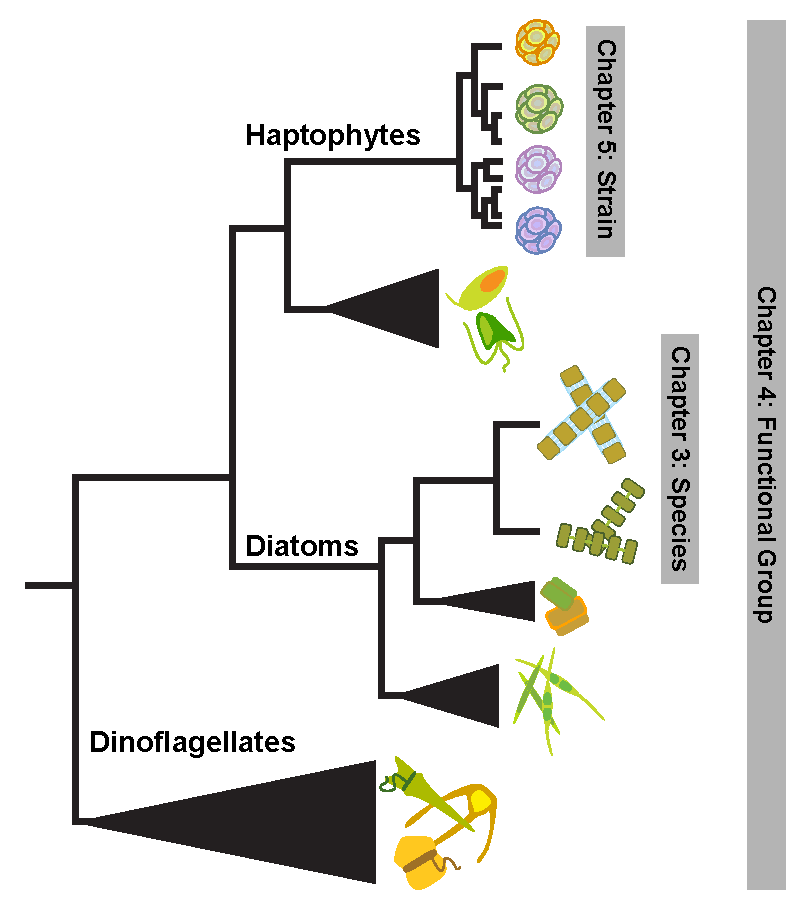
\includegraphics[width=.7\textwidth]{Images/C1_ThesisDiagram.pdf}
    \caption{Conceptual overview of the levels of diversity explored in chapters 3, 4, and 5 of this thesis.}
  \label{fig:c1f1}
\end{figure}


The vast diversity of the phytoplankton has long perplexed biological oceanographers, as these organisms superficially appear to coexist in an isotropic environment while competing for the same basic resources, nutrients and light, thus violating Gause's law of competitive exclusion \citep{Hardin1960}. Niche partitioning of resources has been hypothesized to be one factor enabling the ``paradox of the plankton'' \citep{Hutchinson1961} but quantitative approaches to identify and track it in the field have been lacking. Working at the long-term sampling site in Narragasett Bay, where seasonal dynamics in phytopankton abundances are well-described and where multiple species are known to simultaneously co-exist, metatranscriptome profiling was used to track species-specific metabolic profiles (Chapter \ref{chap:3}. In addition to tracking known metabolic pathways, new techniques were developed to 1) identify novel resource responsive gene targets without a priori knowledge of function and 2) contextualize expression signals to compare the ecophysiology of organisms. This study demonstrated clearly demonstrated fundamental differences in nutrient utilization between two dominant diatom species in the same environment, suggesting that resource partitioning occurring in the field.\par 

Both chapters \ref{chap:4} and \ref{chap:5} focused on characterizing physiological constraints on the oligotrophic eukaryotic phytoplankton, though at different levels of taxonomic resolution. It has been postulated that the net oxygen state of oligotrophic systems is controlled by aperiodic bursts of production by the large eukaryotic phytoplankton in response to nutrient pulses \citep{Karl2003}. Long-term monitoring at Station ALOHA has suggested seasonality in ecosystem productivity, as evidenced by increased carbon and biogenic silica export during summer. Currently, however, very little is known about the nutritional constraints and metabolic capabilities of the three major phytoplankton functional groups in the oligotrophic ocean: diatoms, haptophytes, and dinoflagellates. By sampling and comparing the global gene expression of eukaryotic community both in situ and in simulated deep water upwelling incubations (Chapter \ref{chap:4}), I was able to identify 1) specific drivers of production for taxonomic groups and 2) transcriptional patterns consistent with the previously defined ecological traits and strategies of different functional groups \citep{Margalef1978}. \par

As can be seen from chapters \ref{chap:3} and \ref{chap:4} as well as other published works \citep{Dyhrman2006, Dyhrman2012, Wurch2011, Bertrand2012a, Jones2013, Bender2014, Frischkorn2014}, metabolic plasticity (as measured through proteomic- and transcriptomic-approaches) in response to environmental change is currently a standard means of examining and characterizing physiological responses to perturbation. In the environment, another means of dealing with perturbation is through succession of species or, in some cases, strains. Genomic surveys of cultured isolates of \textit{Emiliania huxleyi} have shown a high level of variability amongst the genomes (Read et al., 2013), which mirrors the physiological variability observed in the field and laboratory as well as its cosmopolitan distribution across oceanic biomes. Using a metatranscriptomic approach, the relative strain composition and metabolic response of \textit{E. huxleyi} was tracked across field observations and in microcosm studies, which shifted the nutrient environment (Chapter \ref{5}). Results demonstrated that the population was constrained by N-limitation. The addition of N produced shift in metabolism that was highly conserved both across replicated experiments and previous culture-based studies. Additionally, changes in strain-specific gene sets point to a shift in the strain composition of the \textit{E. huxleyi} species complex. 
